%% For double-blind review submission, w/o CCS and ACM Reference (max submission space)
\documentclass[sigplan,10pt,review]{acmart}
\settopmatter{printfolios=true,printccs=false,printacmref=false}
%% For double-blind review submission, w/ CCS and ACM Reference
%\documentclass[sigplan,review,anonymous]{acmart}\settopmatter{printfolios=true}
%% For single-blind review submission, w/o CCS and ACM Reference (max submission space)
%\documentclass[sigplan,review]{acmart}\settopmatter{printfolios=true,printccs=false,printacmref=false}
%% For single-blind review submission, w/ CCS and ACM Reference
%\documentclass[sigplan,review]{acmart}\settopmatter{printfolios=true}
%% For final camera-ready submission, w/ required CCS and ACM Reference
%\documentclass[sigplan]{acmart}\settopmatter{}


%% Conference information
%% Supplied to authors by publisher for camera-ready submission;
%% use defaults for review submission.
\acmConference[CMPUT 416 Project Final Document]{}{December 2020}{Edmonton, AB, Canada}
\acmYear{2020}
\acmISBN{} % \acmISBN{978-x-xxxx-xxxx-x/YY/MM}
\acmDOI{} % \acmDOI{10.1145/nnnnnnn.nnnnnnn}
\startPage{1}

%% Copyright information
%% Supplied to authors (based on authors' rights management selection;
%% see authors.acm.org) by publisher for camera-ready submission;
%% use 'none' for review submission.
\setcopyright{none}
%\setcopyright{acmcopyright}
%\setcopyright{acmlicensed}
%\setcopyright{rightsretained}
%\copyrightyear{2018}           %% If different from \acmYear

%% Bibliography style
\bibliographystyle{ACM-Reference-Format}
%% Citation style
%\citestyle{acmauthoryear}  %% For author/year citations
%\citestyle{acmnumeric}     %% For numeric citations
%\setcitestyle{nosort}      %% With 'acmnumeric', to disable automatic
                            %% sorting of references within a single citation;
                            %% e.g., \cite{Smith99,Carpenter05,Baker12}
                            %% rendered as [14,5,2] rather than [2,5,14].
%\setcitesyle{nocompress}   %% With 'acmnumeric', to disable automatic
                            %% compression of sequential references within a
                            %% single citation;
                            %% e.g., \cite{Baker12,Baker14,Baker16}
                            %% rendered as [2,3,4] rather than [2-4].


%%%%%%%%%%%%%%%%%%%%%%%%%%%%%%%%%%%%%%%%%%%%%%%%%%%%%%%%%%%%%%%%%%%%%%
%% Note: Authors migrating a paper from traditional SIGPLAN
%% proceedings format to PACMPL format must update the
%% '\documentclass' and topmatter commands above; see
%% 'acmart-pacmpl-template.tex'.
%%%%%%%%%%%%%%%%%%%%%%%%%%%%%%%%%%%%%%%%%%%%%%%%%%%%%%%%%%%%%%%%%%%%%%


%% Some recommended packages.
\usepackage{booktabs}   %% For formal tables:
                        %% http://ctan.org/pkg/booktabs
\usepackage{subcaption} %% For complex figures with subfigures/subcaptions
                        %% http://ctan.org/pkg/subcaption

%% For drawing graphs
\usepackage{tikz}
\usetikzlibrary{automata, positioning, shapes, fit}

\begin{document}

%% Title information
\title{Visualizing CodeQL Queries in Visual Studio Code}         %% [Short Title] is optional;
%% when present, will be used in
%% header instead of Full Title.
%\titlenote{with title note}             %% \titlenote is optional;
%% can be repeated if necessary;
%% contents suppressed with 'anonymous'
%\subtitle{Subtitle}                     %% \subtitle is optional
%\subtitlenote{with subtitle note}       %% \subtitlenote is optional;
%% can be repeated if necessary;
%% contents suppressed with 'anonymous'


%% Author information
%% Contents and number of authors suppressed with 'anonymous'.
%% Each author should be introduced by \author, followed by
%% \authornote (optional), \orcid (optional), \affiliation, and
%% \email.
%% An author may have multiple affiliations and/or emails; repeat the
%% appropriate command.
%% Many elements are not rendered, but should be provided for metadata
%% extraction tools.

%% Author with single affiliation.
\author{Jacob Skitsko}
%\authornote{with author1 note}          %% \authornote is optional;
%% can be repeated if necessary
\orcid{nnnn-nnnn-nnnn-nnnn}             %% \orcid is optional
\affiliation{
  %\position{Position1}
  %\department{Department1}              %% \department is recommended
  \institution{University of Alberta}            %% \institution is required
  %\streetaddress{Street1 Address1}
  %\city{City1}
  %\state{State1}
  %\postcode{Post-Code1}
  %\country{Country1}                    %% \country is recommended
}
\email{jskitsko@ualberta.ca}          %% \email is recommended

%% Author with two affiliations and emails.
\author{Robert MacGillivray}
%\authornote{with author2 note}          %% \authornote is optional;
%% can be repeated if necessary
%\orcid{nnnn-nnnn-nnnn-nnnn}             %% \orcid is optional
\affiliation{
  %\position{Position2a}
  %\department{Department2a}             %% \department is recommended
  \institution{University of Alberta}           %% \institution is required
  %\streetaddress{Street2a Address2a}
  %\city{City2a}
  %\state{State2a}
  %\postcode{Post-Code2a}
  %\country{Country2a}                   %% \country is recommended
}
\email{rmacgill@ualberta.ca}         %% \email is recommended

%% Author with two affiliations and emails.
\author{Cijie Xia}
%\authornote{with author2 note}          %% \authornote is optional;
%% can be repeated if necessary
%\orcid{nnnn-nnnn-nnnn-nnnn}             %% \orcid is optional
\affiliation{
  %\position{Position2a}
  %\department{Department2a}             %% \department is recommended
  \institution{University of Alberta}           %% \institution is required
  %\streetaddress{Street2a Address2a}
  %\city{City2a}
  %\state{State2a}
  %\postcode{Post-Code2a}
  %\country{Country2a}                   %% \country is recommended
}
\email{cijie@ualberta.ca}         %% \email is recommended



%% Abstract
%% Note: \begin{abstract}...\end{abstract} environment must come
%% before \maketitle command
\begin{abstract}
  CodeQL is a program analysis tool developed by Semmle. Developers and researchers can identify software vulnerabilities and bugs with CodeQL by writing queries in a language called QL. They have also developed CodeQL for Visual Studio Code, which is an open source Visual Studio Code extension written in TypeScript, utilizing CodeQL libraries for analysis. This extension currently displays the analysis results in the tabular view.
  \newline
  \indent In this paper, we present CodeQLVis - a CodeQL visualization tool integrated in Visual Studio Code which creates intuitive graphical representations of the analysis results from CodeQL.

\end{abstract}


%% 2012 ACM Computing Classification System (CSS) concepts
%% Generate at 'http://dl.acm.org/ccs/ccs.cfm'.
\begin{CCSXML}
  <ccs2012>
  <concept>
  <concept_id>10011007.10011006.10011008</concept_id>
  <concept_desc>Software and its engineering~General programming languages</concept_desc>
  <concept_significance>500</concept_significance>
  </concept>
  <concept>
  <concept_id>10003456.10003457.10003521.10003525</concept_id>
  <concept_desc>Social and professional topics~History of programming languages</concept_desc>
  <concept_significance>300</concept_significance>
  </concept>
  </ccs2012>
\end{CCSXML}

\ccsdesc[500]{Software and its engineering~General programming languages}
\ccsdesc[300]{Social and professional topics~History of programming languages}
%% End of generated code


%% Keywords
%% comma separated list
\keywords{Program Analysis, Developer Tools, Visualization}  %% \keywords are mandatory in final camera-ready submission


%% \maketitle
%% Note: \maketitle command must come after title commands, author
%% commands, abstract environment, Computing Classification System
%% environment and commands, and keywords command.
\maketitle


\section{Introduction and Motivation}
CodeQL is a powerful code analysis engine that supports many mainstream programming languages such as Java, C\#, Python, JavaScript and more. Developers are able to use CodeQL to quickly perform data-flow analyses on their programs and identity software vulnerabilities such as taint flows, or to acquire programs' properties such as call graphs.
\newline
\indent Existing tools leveraging CodeQL on the market display the analysis results only in text-based methods, which is not very straightforward and requires users to have knowledge in program analysis to understand. For example, LGTM has tools that make it easier to understand data-flow analysis performed with CodeQL. The way they explore data-flow paths is with a series of code snippets. CodeQL Visual Studio Code extension only outputs the analysis results in tabular view.
\newline
\indent Semmle, the company behind CodeQL, was acquired by GitHub in 2019 and there has been widespread public support for CodeQL's novel approach to static analysis \cite{Semmle_GitHub}. The popularity of this tool, and the lack of visualization support, has given us reason to explore this problem. We've narrowed our scope in this domain to visualizing data-flow analysis, particularly as it pertains to taint-flow tracking.
\newline
\indent Therefore, in order to convey a complete and intuitive picture of a system more quickly than text-based methods, we have extended the CodeQL for Visual Studio Code extension to support taint-flow graph visualizations.

\section{Background}

\subsection{CodeQL}
CodeQL is a tool for performing static analysis that transforms code into queryable relational databases \cite{Semmle_CodeQL_About}. Database queries are then written in the QL language to retrieve certain properties about the code that the database was derived from. This approach makes CodeQL incredibly fast, though the powerful and flexible nature of database queries means that it can be difficult to know exactly what data will have been retrieved and thus, how to visualize it, ahead of time.
\newline
\indent Two queries with the same semantic meaning can retrieve sets of data that are superficially different before processing or manual review. As a result, there are efforts underway to produce libraries of pre-defined queries to help users look for common security vulnerabilities or other issues in their code-base \cite{Semmle_LGTM}. The most-used source is LGTM, a service developed by Semmle and supported by GitHub Security Lab \cite{GitHub_SecurtyLab_CodeQL}.

\subsection{Visual Studio Code Extensions}
Visual Studio Code extensions are in-editor tools that are created by their community of users. Visual Studio Code, often abbreviated to VS Code, offers a powerful Extension API for this purpose. Extensions are written in JavaScript or TypeScript and can modify almost any aspect of VS Code. Features such us simple editor themes, all the way to adding support for self-developed programming languages is possible.
\newline
\indent Of particular interest for our purposes are VS Code Webviews. Where an extension that has been limited to the Extensions API are limited to modifying existing elements of the editor, the Webview API provides an opportunity to render interactive HTML in order to create entirely new functionality within the editor. CodeQL for Visual Studio Code, for example, uses this API to render query results as tables of data.

\section{Overview}
Since the CodeQL for Visual Studio Code extension is open source, we created a fork of the public repository in order to modify the extension such that graphical visualization would be possible. After completing a query, we pass processed data to a modified fork of a second open source extension, VS Code Debug Visualizer. This process relies on the VS Code Webview API and related libraries that drive graph visualization in that environment.
\newline
\indent CodeQLVis is provided as supplemental functionality to the base CodeQL VS Code extension's default way of rendering the results in tabular view. Users select which functionality they would like to employ with simple context-menu options. Further implementation details follow.

\begin{figure}[H]
  \centering
  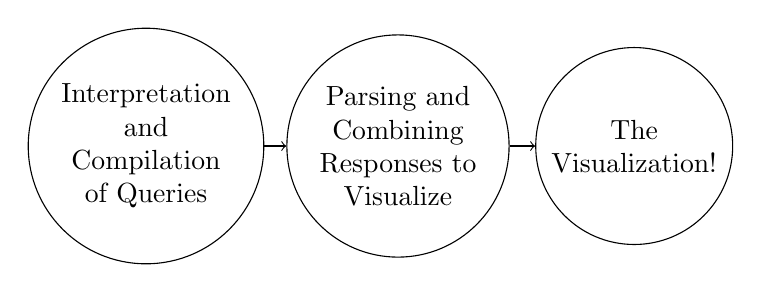
\begin{tikzpicture}[node distance = 3cm,on grid,auto,align=center, minimum size=6cm]
    \node[state] (a) {Interpretation \\and \\Compilation \\of Queries};
    \node[state] (b) [right = of a, xshift=0.2cm] {Parsing and \\Combining \\Responses to \\Visualize};
    \node[state] (c) [right = of b] {The \\Visualization!};
    \path[->]
    (a) edge (b)
    (b) edge (c)
    ;
  \end{tikzpicture}
  \caption{The work flow}
\end{figure}

\section{Approach}

\subsection{CodeQL Queries}
Our approach is to make multiple CodeQL queries derived from the original query to get relevant information. It would be possible to accomplish this with a single query, but that would require modifying the CodeQL command line to get new information, thus reducing our compatability across different programming languages and operating systems. Using multiple queries instead maintains this compatability, at the cost of a small increase in runtime.
\newline
\indent We utilize existing CodeQL infrastructure from the CodeQL extension as much as we can. This also means that (with slightly more effort) we could incorperate CodeQLVis into existing CodeQL extension elements, such as query history. At the moment any queries we make with CodeQLVis can be recalled as CodeQL queries using the history manager, but we do cannot recall them to redisplay visualized queries.
\newline
\indent We will make at most three queries with the CodeQL command line for a given CodeQLVis visualization. The first will be the unmodified original query. If the original query had a sanitizer method we will make two additional queries modified from our original query: one where we remove the sanitization from our query, and one where we replace the sink detection in our query with what was formerly the sanitization detection. The first of these modified queries will tell us when we have sink nodes that would have been tainted, if not for the sanitization we have. The second of these modified queries tells us how far taint flows before being sanitized. Figure \ref{queries} shows the information the different queries find.
\newline
\begin{figure}[H]
  \centering
  \begin{tikzpicture}[node distance = 1.5cm,on grid,auto]
    \node[state] (s1) {$s_1$};
    \node[state] (s2) [right = 2cm of s1] {$s_2$};
    \node[] (v1) [below = 3cm of s1] {$\vdots$};
    \node[] (u1) [below = of s2] {$\vdots$};
    \node[state] (v2) [below = of u1] {$v$};
    \node[] (u2) [below = of v2] {$\vdots$};
    \node[state] (t1) [below = 6cm of s1] {$t_1$};
    \node[state] (t2) [below = 6cm of s2] {$t_2$};

    \node[draw,densely dotted,fit=(s1) (v1) (t1)] {};
    \node[draw,densely dotted,fit=(s2) (v2)] {};
    \node[draw,loosely dashed,fit=(s2) (v2) (t2)] {};

    \node[below = of t2, xshift=-0.75cm] {$
        \begin{matrix}
          s_1,s_2: & \text{source nodes}    \\
          v:       & \text{sanitizing node} \\
          t_1:     & \text{tainted sink}    \\
          t_2:     & \text{untainted sink}  \\
        \end{matrix}
      $};
    \path[->]
    (s1) edge (v1)
    (v1) edge [shorten <= 5pt] (t1)
    (s2) edge (u1)
    (u1) edge [shorten <= 5pt] (v2)
    (v2) edge [dashed] (u2)
    (u2) edge [shorten <= 5pt,dashed] (t2)
    ;
  \end{tikzpicture}
  \caption{Query diagram}
  \label{queries}
\end{figure}
 Figure \ref{queries} represents an example where taint flows from the source $s_1$ to the sink $t_1$, but taint flow from the source $s_2$ is blocked by $v$ before it reaches the sink $t_2$. The dotted box around $s_1,t_1$ represents our first query. The dashed box around $s_2,v,t_2$ represents our second query. The dot-dashed box around $s_2,v$ represents our third query. These queries gives us the information for where taint has reached sinks, where it could have reached a sink if it had not been sanitized (by $v$), and where the taint was sanitized.

\subsection{Queries to Graphs}
Once we have obtained information from our queries we can construct a graph that represents how taint flows. In the future, this graph can be adapted to various styles of visualization - the same underlying graph can be used to render different visualizations.
\newline
\indent To construct our graph we first add all of the results from our original query. This represents when taint has flown from sources to sinks. If our modified queries have been made (i.e. the original query had a sanitizer method) we use our second query to find all paths from sources to sinks where taint could have flown undisrupted if not for our sanitization. Finally, we use our third query to determine paths from sources to sanitizing nodes where taint has been blocked. This tells us how far taint flows on the paths provided by our second query. Combining the results from each of our queries we get a graph that has all paths where taint flows from sources to sinks, and all paths where taint would have flowed if not for sanitization, including how far the taint does flow. Of course, we combine nodes referencing the same locations in code so we may accurately depict cases such as when a source acts as a source of taint for distinct sinks.

\subsection{Rendering Results}

\begin{figure}[h]
  \centering
  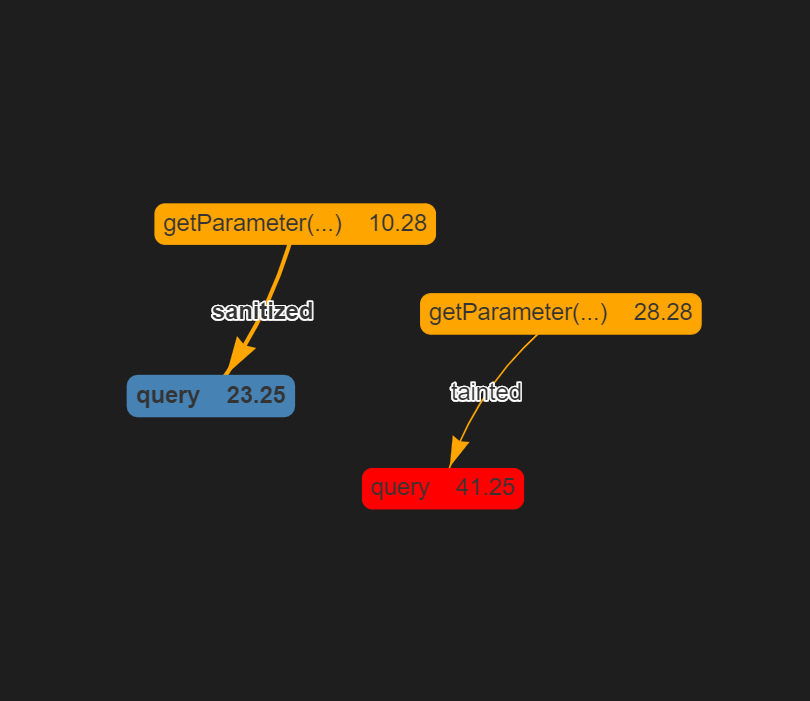
\includegraphics[width=\linewidth]{taint_part}
  \caption{Taint analysis visualization only showing sources and sinks. Orange denotes a source matching the query. Red denotes a tainted sink. Dark blue denotes a sink that is sanitized.}
\end{figure}

\begin{figure}[h]
  \centering
  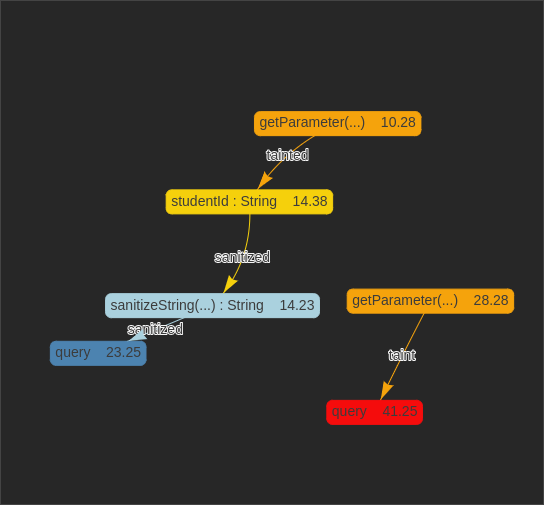
\includegraphics[width=\linewidth]{taint_full}
  \caption{Taint analysis visualization with full data-flow path. Yellow denotes data that is tainted. Light blue denotes data that is no longer tainted.}
\end{figure}

The rendering part of the visualization tool is running on the Webview infrastructure of VS Code. The React.js framework is used to build the front-end of CodeQLVis. The TypeScript library hediet/visualization is used as the rendering infrastructure for the graphs. Websocket infrastructure enables the back-end to send analysis results to the front-end for rendering.
\newline
\indent This functionality has been made available through the open source VS Code Debug Visualizer extension. Our modifications allowed us to control data-input from the CodeQL extension via a new extension command that take file-paths to JSON data as arguments. This JSON data is of the format outlined in the previous section.
\newline
\indent We have also written some support classes and modified existing classes to better represent our tool and provide a smooth in-editor user experience. These classes offer some control over the state of the extension, preventing the user from performing actions that may otherwise cause instability.

\section{Evaluation}
Due to the nature of this project, we only examined whether CodeQLVis generates correct taint-flow graphs. Therefore, we tested CodeQLVis with different code examples from the official CodeQL documentation and compared our taint-flow graphs with the CodeQL analysis results through manual inspections. In particular, we ask the following questions.
\newline
\newline
\textbf{5.1. Are the roles of nodes on taint-flow graphs correctly labeled? }
\newline
Nodes on the visualization graphs have their roles - \textbf{Source, Sink, Sanitizer, Tainted Variable and Untainted Variable}. CodeQLVis should not label any node in an incorrect role.
\newline
\newline
\textbf{5.2. Are there any missing taint-flow paths? }
\newline
CodeQLVis should display all the taint-flow paths identified by CodeQL.
\newline
\newline
\textbf{5.3. Are there any redundant taint-flow paths? }
\newline
CodeQLVis should not display any false taint-flow path.
\newline
\newline
\textbf{5.4. Are the nodes on the taint-flow path in correct order? }
\newline
CodeQLVis should display the nodes in the exact order in their taint-flow paths as the analysis results generated by CodeQL.
\newline
\newline
We observed no contradictions between our visualization graphs and CodeQL analysis results.

\section{Future Work}
CodeQLVis is the first visualization tool for CodeQL that does not rely on textual or tabular representation. It provides intuitive means of understanding the analysis results generated by CodeQL. Also, it is integrated into the existing CodeQL for Visual Studio Code extension, so developers can benefit from this tool in conjunction with existing methods. However, we admit that this tool has room for a number of improvements and additional features. There is a large space of possibilities for future development efforts.
\newline
\indent The graphs can be more interactive. Users should be able to navigate between the code snippets by clicking on the nodes on the visualization graphs. In addition, large graphs can become crowded due to the amount of information represented by labels on the nodes. We are of the opinion that interactive functionality, such as hover-text, could provide more complete information while keeping the nodes themselves small and concise. This, however, will only be achievable if the current visualization process is removed in favour of a more powerful, customizable, library. Should the visualization library be replaced, this would also open up opportunities for richer visualizations.

\begin{figure}[h]
  \centering
  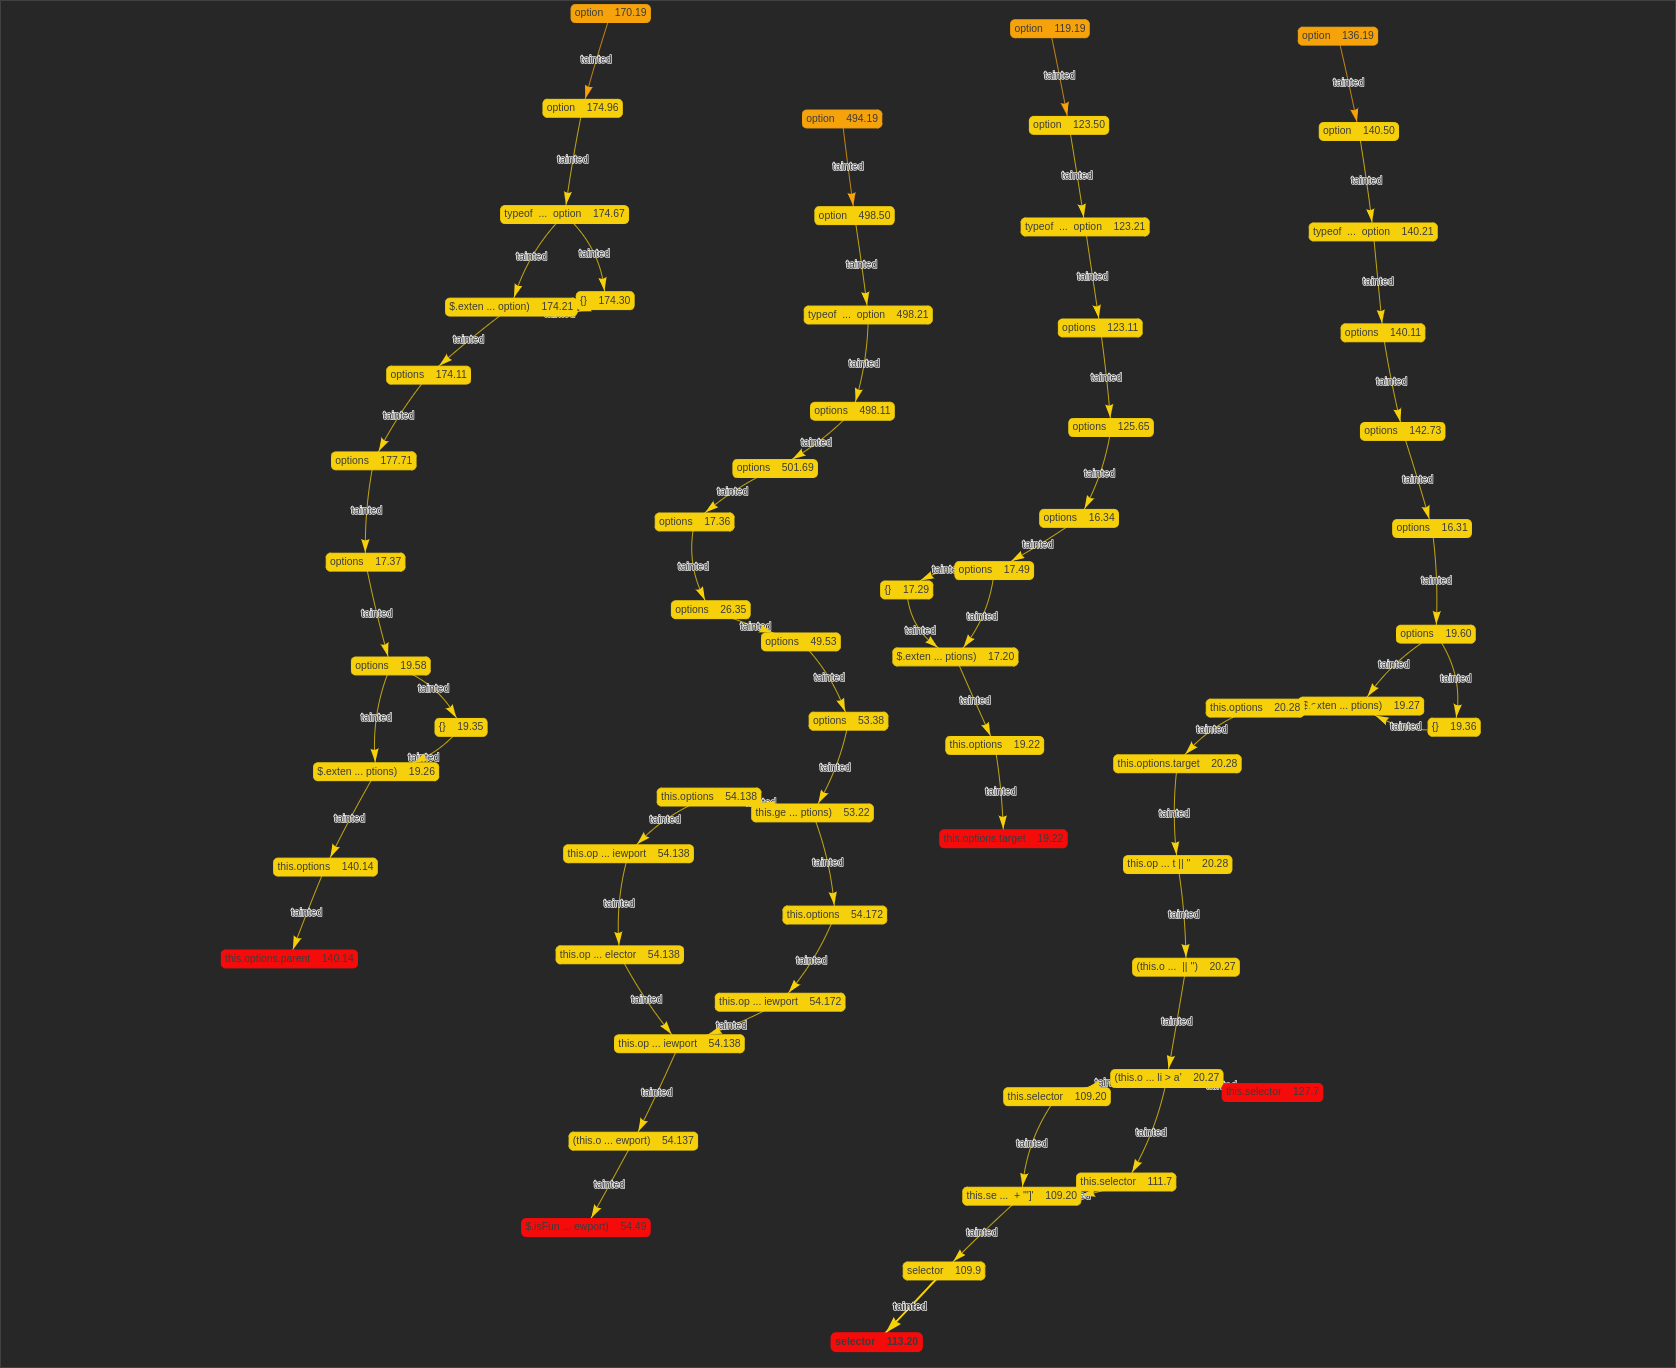
\includegraphics[width=\linewidth]{large_taint_full}
  \caption{Taint analysis over a large domain with full visualization.}
\end{figure}

\indent Our visualization tool only supports taint-flow analysis. More specifically, it only supports taint-flow analysis driven by queries with a limited format. While we do pre-process queries to make modifications that help our visualization effort, this simply isn't sustainable over the limitless query formats users could use. We propose curating query templates in a similar format to those found on LGTM in order to limit the space of queries we have to deal with. This would also lay the groundwork to develop other categories of analysis that could receive visualization support. Graphing dead-code analysis, for example, could better contextualize those results.

\section{Related Work}
There has been a wealth of work done in the space of visualizing data-flow analysis, which can be considered a superset of taint-flow analysis. There has been less work specifically on visualizing taint-flow, and none specifically in our area of interest. We highlight some efforts that have the most overlap with our project.
\newline\newline
\indent \textbf{"Understanding and Visualizing Full Systems with Data Flow Tomography"} \cite{10.1145/1353535.1346308} outlines an approach whereby data is tagged and tracked through the program to develop a visualization of all interconnected pieces. In contrast, rather than doing live analysis, we use CodeQL to perform static analysis and find theoretical data-flow paths that meet certain pre-defined criteria.
\newline\newline
\indent \textbf {VisuFlow} \cite{10.1145/3183440.3183470} is a plugin developed for Eclipse that generates visualizations for static analysis performed by Soot. While similar to our work, and interesting as a proof-of-concept, their plugin operates in a different context using a different engine for analysis.
\newline\newline
\indent \textbf {CodeSonar} is a commercial program analysis tool developed by GrammaTech, Inc. It supports taint analysis visualization for several languages. It can be integrated into Eclipse, IDEA and Android Studio. However, this product is not free to use so we are not able to comment at length about it.

\section{Conclusion}
We have shown a possible route to extend CodeQL for Visual Studio Code, offering a more intuitive and straightforward visual representation of data that is otherwise typically presented in tabular format. This optional visualization has been further broken down into different levels of granularity per a user's preference for a given query. Our approach leverages the source extension such that we can interpret taint-flow analysis queries of specific formats, subtly modifying queries before execution where necessary.
\newline
\indent
CodeQLVis is presented as a proof-of-concept work rather than a perfect program analysis visualization tool. We believe there is a huge space for improvements in the future, such as supporting more program analysis visualizations, enabling more interactions between the developers and the graphs and making it more friendly for people without fundemental program analysis knowledge. 

\bibliography{codeql-vis-refs}

\end{document}
